
\section{Experiments}
We applied our implementation to both concept learning task from the original paper: the \textit{Letter Arithmetic} task and the \textit{Number Game}. 
As we were interested in the method and its possible applications, we performed simulations only and no experiments with humans.
%What follows is a brief description of the tasks, our simulation approach and an explanation of our results.

\subsection{Baselines}

We compare the results to the baselines introduced in the original paper: a \textit{random} policy, a random policy with only quiz and example actions (\textit{quiz-example only/QE only}) and policy with planning according to \textit{maximum information gain (MIG)}.

% TODO check, filtering
The \textit{random} policy selects any of the $a \in A$ actions randomly, however, making sure that no item $i \in I$ is sampled twice in the same teaching phase.
%In the \textit{number game}, there are some further constraints that are applied to the randomness.


The \textit{quiz-example only} policy ignores the feedback activity.
It was introduced since in the first original experiment with the letter arithmetic task, the planning algorithms did not use any feedback actions, resulting in a much higher average cost for the random policy compared to the POMDP planners.

The \textit{maximum information gain} policy performs a single planning step with the continuous learner model. For every possible action, it simulates the belief change according to the continuous model and compares the Shannon entropy of the current and the new belief state.

\begin{equation}
    entropy(b)=\sum_{s_p \mid p \in P}{w_{s_p}} \cdot \left( -\sum_{h \in H}{p_{s_p}(h) \cdot \ln\left( p_{s_p}(h) \right)} \right)
\end{equation}

The planner selects the action which produces the highest information gain for the learner, i.e., the one that reduces the entropy the most.
As with the continuous policy, the particle filter approximation is employed, and thus, the entropy of the belief state is calculated as the weighted sum over the entropy of the particles.
This policy provides only example activities to teach a concept as refinement activities do not provide new information to reduce the entropy.
As such, it cannot understand errors during learning and revise its belief.


\subsection{Task 1: Letter Arithmetic}

The \textit{letter arithmetic} task is composed of addition equations with two letters, such as $A+B=3$. In the original experiments, the mapping length is set to 6, which corresponds to the letters A-F being mapped to the numbers 0-5 (we confirmed that there was a typo in one passage noting a larger range of numbers 0-6).

Some sample actions are thus: $B+F=5$ (example), $A+C=?$ (quiz) and followed by $correct$ or $answer=2$ for feedback actions. 
The number of possible teaching items $I$ can be reduced by only considering the possible combinations of the letters, i.e., ignoring order. For the case with 6 letters, this gives $|I|=15$ and a maximum $|I \times T|=45$ actions to evaluate.

The set of valid responses $Z$ are the numbers $1-9$.
During the assessment phase, the learner is queried to provide the correct mapping for each letter.
The estimation of the belief value of the leaf nodes $\Hat{V}(b)$ follows \autoref{eq:leaf-calc} with $\alpha=10$.
We use the original values for the cost function $C(a)$ and noise parameters, as shown in tables \ref{tab:action-cost-t1} and \ref{tab:noise-t1}, that were fitted from control experiments with users in the original study.

\begin{table}
\small
\parbox[t]{.49\linewidth}{
    \centering
    \begin{tabular}[t]{l|r}
        \hline
        \textbf{Teaching type} & \textbf{Cost} in seconds \\
        \hline
        Example & 7.0 \\
        Quiz    & 6.6 \\
        Feedback & 12.0 \\
        \hline
    \end{tabular}
    \caption{\textit{Letter arithmetic}: Teaching activity costs}
    \label{tab:action-cost-t1}
}
\hfill
\parbox[t]{.49\linewidth}{
    \centering
    \begin{tabular}[t]{l|rr}
        \hline
        \textbf{Learner model} & $\epsilon_t$ & $\epsilon_p$ \\
        \hline
        Memoryless  & 0.15 & 0.019 \\
        Discrete    & 0.34 & 0.046 \\
        Continuous  & 0.14 & 0.12 \\
        \hline
    \end{tabular}
    \caption{\textit{Letter arithmetic}: Noise parameters}
    \label{tab:noise-t1}
}
\end{table}


The concept space $H$ is composed of all permutations of the 6 letters mapped to 0-5, so $|H|= 720$. 
This is also the state space for the memoryless and discrete policy, as well as the particle size in the continuous policy.
All concepts are assumed to be equally likely, so a uniform prior $p_0$ over the concepts is used.


\subsection{Task 2: Number Game}

The second task is called \textit{Number Game} \cite{tenenbaum2000rules}. 
The goal in this task is to infer a specific number concept for the number range $1-100$. Such a concept can be either mathematical $H_{math}$, like odd, even, multiples of 5, etc., or a range based concept $H_{range}$, like 10-20 or 64-83.
The student is presented a number and is either told if the number belongs to the target concept (example and feedback activities) or is asked to provide this categorization (quiz and question activities).

The set of teaching items $I$ is the range of numbers $1-100$, resulting in $|I \times T|=300$ possible actions.
The set of possible responses $Z$ only contains two values: `inside' and `outside' the concept.
During the assessment phase, the learner is presented with 10 items and has to give 10 correct answers to display mastery of the concept and terminate the teaching.
Of these items, 5 are sampled from within the concept and 5 from outside the concept.

For $\Hat{V}(b)$ to estimate the belief value of leaf nodes, \autoref{eq:leaf-calc} with $\alpha = 10$ is used as before.
Again, we use the original values for the cost function $C(a)$ and noise parameters, as shown in tables \ref{tab:action-cost-t2} and \ref{tab:noise-t2}, that were fitted from control experiments with users in the original paper.


\begin{table}
\small
\parbox[t]{.49\linewidth}{
    \centering
    \begin{tabular}{l|r}
        \hline
        \textbf{Teaching type} & \textbf{Cost} in seconds \\
        \hline
        Example & 2.4 \\
        Quiz    & 2.8 \\
        Feedback & 4.8 \\
        \hline
    \end{tabular}
    \caption{\textit{Number game}: Teaching activity costs}
    \label{tab:action-cost-t2}
}
\hfill
\parbox[t]{.49\linewidth}{
    \centering
    \begin{tabular}{l|rr}
        \hline
        \textbf{Learner model} & $\epsilon_t$ & $\epsilon_p$ \\
        \hline
        Memoryless  & 0.25 & 0.14 \\
        Discrete    & 0.18 & 0.10 \\
        Continuous  & 0.21 & 0.15 \\
        \hline
    \end{tabular}
    \caption{\textit{Number game}: Noise parameters}
    \label{tab:noise-t2}
}
\end{table}

The exact concept space is more difficult to recover. Tenenbaum \textit{et al.} \cite{tenenbaum2000rules} originally described 5,083 possible concepts. Rafferty \textit{et al.} reported to use 6,412 concepts, but the exact definition is not given. 
We received the original unlabelled concept values from the original author, from which we reverse engineered 6,354 of the 6,412 concepts (the remaining 58 concepts were the same as other concepts, and as there were no labels, we considered them duplicates).
In addition to the original 5,083 concepts, the set of \textit{less probable mathematical concepts} $H_{math+}$ is added, e.g., ``multiples of 4 minus 1'' or larger multiples such as ``multiples of 25''.
Details of the concept space can be found in \autoref{tab:ng-concepts}.

The definition of the prior $p_0$ is following a hierarchical model as described in \cite{tenenbaum2000rules}. 
The mathematical concepts $H_{math}$ and $H_{math+}$ are assigned $\lambda$ of the probability and each class in turn is assigned half of this prior.
As both classes are a lot smaller than the range concepts, they are assigned the majority of the prior if $\lambda$ is not small.
Inside each class, the prior is shared uniformly: $p_0(h \in H_{math}) = 0.5 \cdot \lambda / |H_{math}|= \lambda / 168$ and $p_0(h \in H_{math+}) = 0.5 \cdot \lambda / |H_{math+}|= \lambda / 5048$. 

The remainder $(1 - \lambda)$ is shared among the number range concepts $H_{range}$ proportional to an Erlang distribution according to their interval size: $p_0(h \in H_{range}) \propto (|h|/\sigma^2) \cdot e^{-|h|/\sigma}$. This should capture the intuition that medium sized ranges are more likely than very big or very small ranges.

For the free parameters $\lambda, \sigma$, we use the same values as originally described in \cite{tenenbaum2000rules}: $\lambda = 1/2, \sigma = 10$. 
That means, all mathematical concepts are assigned a prior probability of $1/168 \approx 5.95 \cdot 10^{-3}$, the less probable mathematical concepts a prior of $1/5048 \approx 1.98 \cdot 10^{-4}$, and e.g. the range 1-100 is assigned the prior $\approx 3 \cdot 10^{-7}$ while the range 64-83 a prior of $\approx 1.67 \cdot 10^{-4}$. 

As the less probable mathematical concepts $H_{math+}$ were reverse engineered, the corresponding prior was similarly deduced to best match the associated prior given by the original authors.
Still, these priors slightly differ 5-10\% from our reported values. On the one hand, this is because our space is smaller by 58 items but also because they might have used a slightly different $\lambda$ (for instance, a value around $0.55519$ instead of $1/2$ could explain this difference but it does not change the results significantly).

\begin{table}
\centering
\small
\begin{tabular}{l|r|r}
    \hline
    \textbf{Concept class}  & \textbf{Number of concepts} & \textbf{Prior} \\
    \hline
    \textit{Mathematical concepts (below)} & \textit{42} & $\sum = 1/4$ \\
    \hline
    Odd, even               & 2     & $1/168 \approx 0.0059524$ \\
    Square, cube            & 2     & $1/168$ \\
    Primes                  & 1     & $1/168$ \\
    Multiples of 3-12       & 10    & $1/168$ \\
    Powers of 2-10 (incl. 1)& 9     & $1/168$ \\
    Powers of 2-10 (excl. 1)& 9     & $1/168$ \\
    Numbers ending in 1-9   & 9     & $1/168$ \\
    \hline\hline
    \textit{Less probable mathematical concepts (below)} & \textit{1262} & $\sum = 1/4$ \\
    \hline
    Multiples of 13-50        & 38 & $1/5048 \approx 0.0001981$ \\
    Multiples of 3-50 minus $1...n-1$ & 1224 & $1/5048$ \\
    \hline\hline
    \textit{Ranges n-m}, $1 \leq n \leq 100, n \leq m \leq 100$ & \textit{5,050} & $\sum = 1/2$ \\
    \hline
    E.g. Range 10-20        & 1 & $\approx0.0002262$ \\
    E.g. Range 64-83        & 1 & $\approx0.0001672$ \\
    E.g. Range 1-100        & 1 & $\approx0.0000003$ \\
    ... & &                     \\
    \hline\hline
    \textbf{Total concepts} & \textbf{6,354} & $\sum = 1$ \\
    \hline
\end{tabular}
\caption{Set of concepts for the number game and their corresponding priors.}
\label{tab:ng-concepts}
\end{table}

Finally, the two random policies' sampling strategy is modified such that with 50\% probability an item inside the concept, and otherwise outside the concept is sampled.
This was introduced after the original authors noticed that a completely random policy was too frustrating for the human learners.

\subsection{Simulation}

We validated our implementation by running the same simulations as in the original paper. 
Every planning policy was tested with every learner model simulation. 
Hence, for every simulated learning model, the three baselines and the three planning policies with the learning models were tested, leading to a total of 18 pairings.
Those pairs were run 50 times each with a different but controlled seed set for the random number generators. In all trials of the same pair, the task instance was the same. 
The horizon depth and samples per level were the same as in the original paper.

In the \textit{letter arithmetic} task, all models used a horizon of $d=2$. 
The memoryless model sampled 7 items in the first level and 6 in the second level. The discrete model with memory sampled 8 items in both levels, and the continuous model sampled respectively 4 and 3 items.
Teaching phases consist of three actions followed by an assessment phase. After a maximum of 40 teaching phases (i.e., 120 total actions) and a failed assessment phase, the learning was terminated without success.

In the \textit{number game}, the memoryless model and the discrete model used a horizon of $d=2$, with 6 and 8 items sampled, and 6 items sampled in both levels respectively. The continuous model had a horizon of $d=3$, with 6, 6 and 8 items sampled. 
Teaching phases lasted 5 actions. The maximum number of teaching phases was again 40 (i.e., 200 total actions).

In both tasks, the memory model was using a memory size of 2, and the continuous model's maximum particle size was set to 16 with the particle depletion threshold of 0.005, as in the original experiments.
% try in a big table everything

\subsubsection{Precomputing actions}
The authors note that for computational reasons, they precomputed the first actions and cached them to be used in all trials. During this precomputation, 10 items were sampled per level.
The original paper reports only this number for the first task, but we used the same number for the second task. In the \textit{letter arithmetic} task, 9 actions were precomputed, while in the \textit{number game}, 20 actions were precomputed.
Also, the same horizon as the target policy is used in every step.

Through precomputing actions, possibly better starting points would be found. Naturally, during precomputation, the true responses of the learners are not known.
If an action with a non-empty response set is returned as the best action, a separate branch for every possible response has to be followed.
This ensures that during teaching, the corresponding path according to the learner's response is available.
This leads to a possibly very large number of branches.

\subsubsection{Evaluation metric}

To compare our replication, we use the same metric as in the original study to evaluate the planning policies for each simulated learner, the \textit{median time to mastery}.
This refers to the hypothetical time the simulated learner spends with the automated teacher based on the time cost of each action type.

For example, in the letter arithmetic task, if a learner is shown three examples and one quiz, the expected time to mastery is $27.6$. 
Note that assessment phases are not taken into consideration in the time calculation.
If mastery is not achieved, the total time spent until this point is used. 
As each teaching phase consists of 3 actions and the least costly activity is the quiz, the theoretical minimum time is $19.8$ (although it is impossible to learn only via quizzes), and the maximum time would be $1440$. 
In a setting using only examples, the minimum time would be $21.0$, while for maximum runs, averaging over the action costs, the time until termination is expected to be $1024$.


For the number game, the action costs are much smaller, while the teaching phases are longer.
The theoretical minimum time is $12.0$ using example activities.
The averaged maximum in this task is then $\approx 666.67$.

These numbers allow us to get an intuition of how well a learner is doing in respect to the bounds of the problem.

\subsection{Results}

\subsubsection{Letter Arithmetic}

% \begin{figure}
%     \centering
%     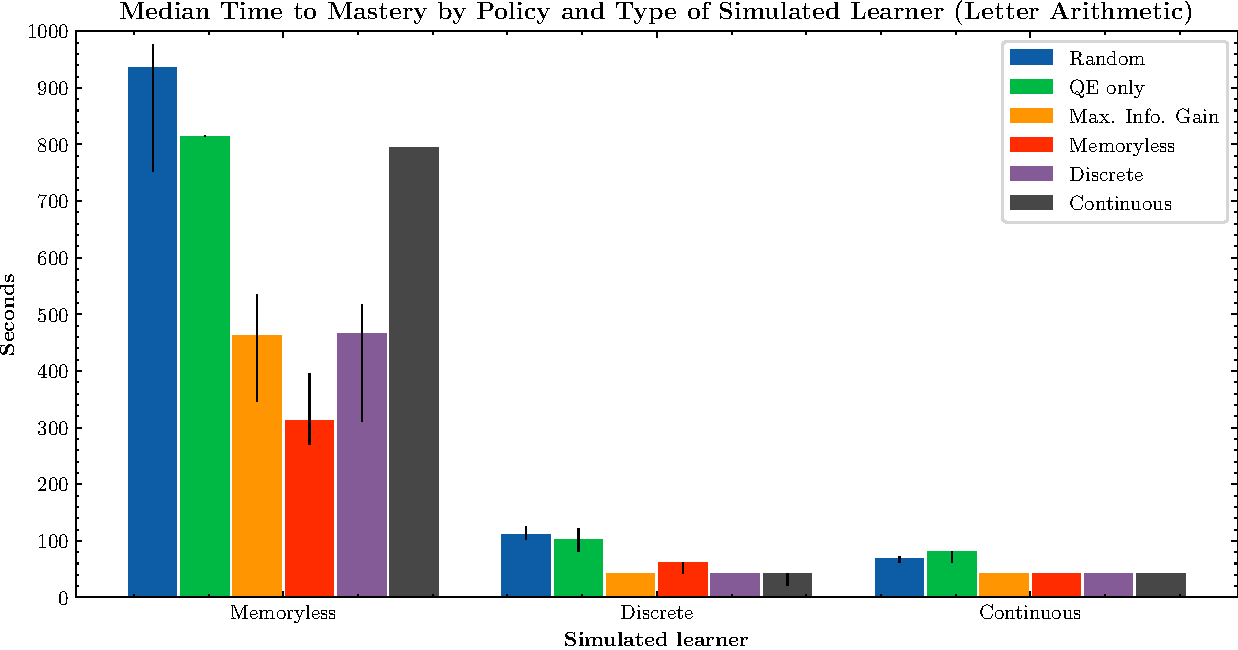
\includegraphics[width=\linewidth]{median-time-letter.pdf}
%     \caption{Median time to mastery for the letter arithmetic task. The results are grouped for each simulated learner (x axis) showing the performance of the different policies. The error bars represent the bootstrapped 68\% confidence interval. Replication of figure 4 from the original paper.
%     %The results are similar as well. Our results differ for the simulated memoryless learner which achieves a significantly better score for the memoryless planning model, and a worse score for the discrete memory planning model. Both the simulated learners with discrete memory and the continuous model achieve the same near minimum results with 42.0s, corresponding to two teaching phases with examples.
%     }
%     \label{fig:median-time}
% \end{figure}


% \begin{figure}
%     \centering
%     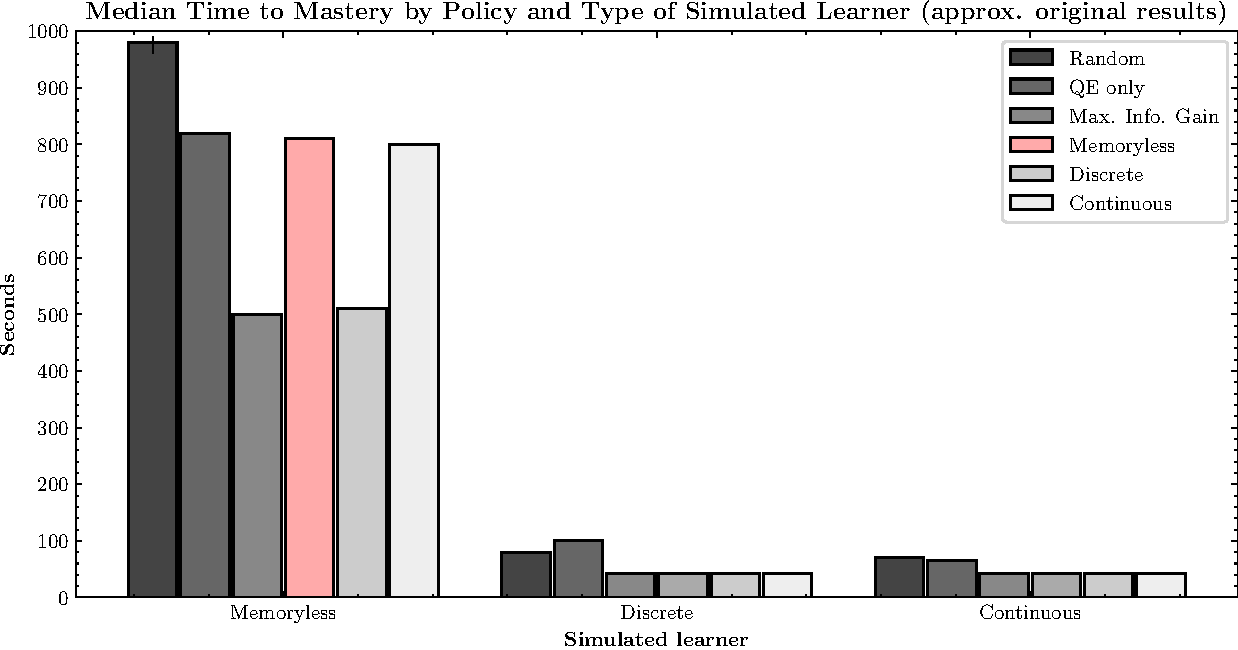
\includegraphics[width=.75\linewidth]{median-time-letter-orig.pdf}
%     \caption{Replicated figure 4 of the original paper for comparison with our results
%     The main difference is highlighted in red.
%     }
%     \label{fig:difference-t1}
% \end{figure}

\begin{figure}[h]
    \centering
    \begin{subfigure}{1\linewidth}
        \centering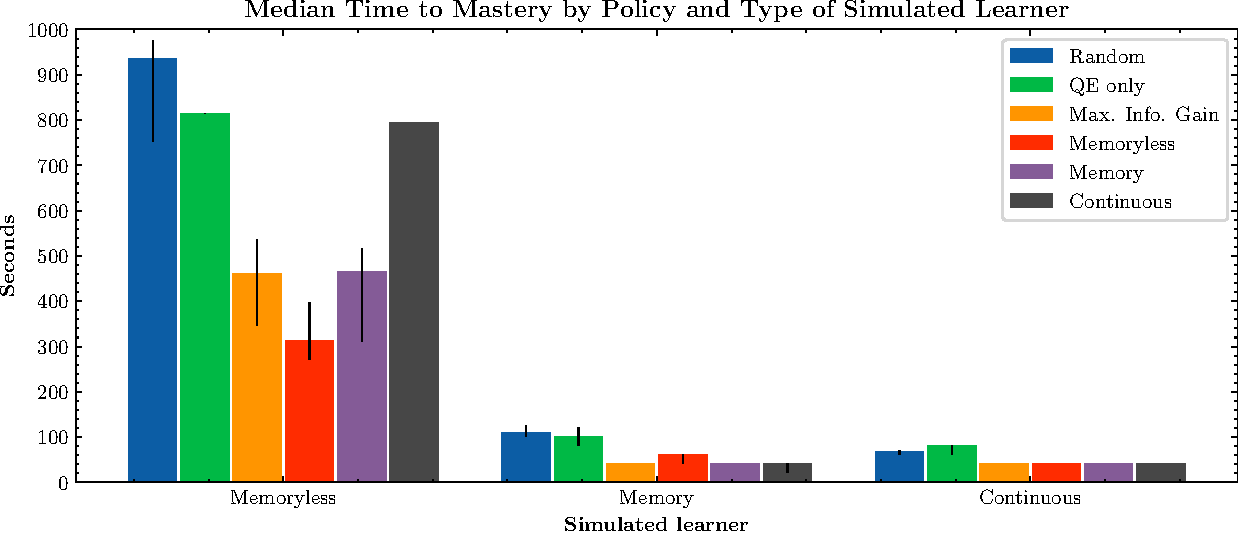
\includegraphics[width=1\linewidth]{figures/median-time-letter-pre.pdf}
        \caption{Our results}
    \end{subfigure}%
    \vspace{10pt}
     
    \begin{subfigure}{1\linewidth}
        \centering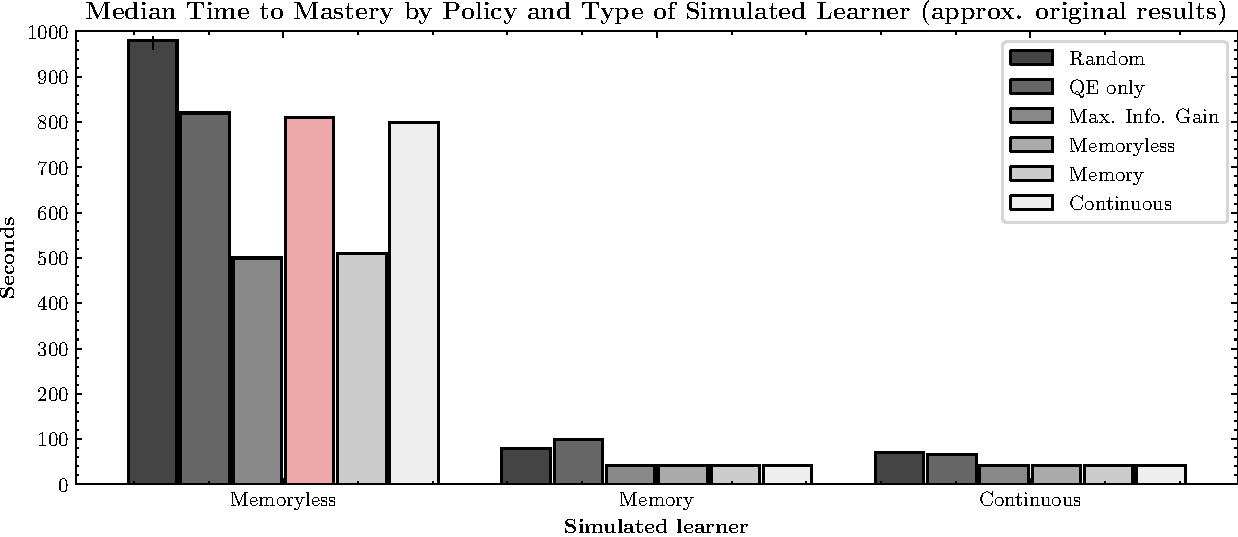
\includegraphics[width=1\linewidth]{figures/median-time-letter-orig-small.pdf}
        \caption{Original results, recreated from the original figure 4. The main difference is highlighted in red.}
    \end{subfigure}
    
    \caption{Median time to mastery for the letter arithmetic task. The results are grouped for each simulated learner (x axis) showing the performance of the different policies. The error bars represent the bootstrapped 68\% confidence interval.
    }
    \label{fig:median-time-comp}
\end{figure}

Our simulation results are shown in \autoref{fig:median-time-comp} (a).
The overall results of the median time to mastery are very similar to the original paper with some notable differences.
%Exact numbers for the original data are not available, so the values given below are approximated from Figure 4 of the original paper. 

Most notably, the result for the memoryless learner with the memoryless policy differs. It is lowest for the memoryless learner with 323.5s while the original authors reported a time around 810s.

The results for the other learners match the original data closely, the random policies differ slightly.
The results for the three planner and the maximum information gain policies paired with the discrete and continuous learners all have a median of 42.0s (two rounds of example activities). 
Only the memoryless policy for the discrete learner deviates from this value, although it is still contained in its confidence interval.

When comparing the time to mastery for the two random policies, note that the QE only policy might achieve a lower number because the most expensive action is not used.
This can have a negative effect on the learning because with the random policy, there is a $2/3$ chance of seeing evidence, while with QE only, there is only a $1/2$ chance. 
This might explain the higher failure rate for the memoryless learner with the QE only policy.


\begin{table}[h]
    \centering
    \small
    \begin{tabular}{l|rrr|r}
        \hline
        \textbf{Policy} & \multicolumn{2}{l}{\textbf{Failure rate with learner}} & & \textbf{Computation time}\\
                        & Memoryless &  Memory & Continuous &  \\
        \hline
        Random          & 50\% & 0\% & 0\% & - \\
        Random QE only  & 68\% & 0\% & 0\% & - \\
        Max. Information Gain & 32\% & 0\% & 0\% & 0.1s \\
        \hline
        Memoryless      & 22\% & 0\% & 0\% & 1.3s \\
        Discrete memory & 18\% & 0\% & 0\% & 2.2s\\
        Continuous      & 96\% & 26\% & 0\% & 1.2s \\
        \hline
    \end{tabular}
    \caption{Failure rates and mean computation times over 50 simulations for each policy-learner pair.
    %Failure is encountered when the concept is not learned after 40 teaching phases.
    }
    \label{tab:failures-t1}
\end{table}

The failure rate of the different simulations, i.e., how many times a learning session was terminated after 40 rounds of teaching phases before the learner achieved mastery of the concept, are reported in \autoref{tab:failures-t1}. 
It shows that the memoryless learner consistently failed to learn the concept, ranging from 18\%-96\% of the cases.
It is highest with the continuous policy at 96\% and second highest for the QE only policy at 68\%. The median time to mastery is very similar in both cases though since the continuous policy samples only the cheapest activity type (quiz) after some point.
The discrete memory learner only fails with the continuous policy in 26\% of the cases, while the continuous learner never fails to learn.
Although the information is not available in the original paper, we assume that the failure rates are similar since the median time to mastery is very close.



\autoref{tab:failures-t1} shows computation times for the different models across all learners. 
%Pre-planning is well below one minute in all cases. 
%However, only one or two paths are considered, as mostly example actions were planned which have no responses to adapt to. 
The online planning computation times are well below 3 seconds which was put forward as the threshold in the original paper. 
%This means, we could increase the sample sizes and stay within the limit.
Increasing the sample sizes did not produce significantly different results. 
%We tested increasing the sample size to 10 for all models and the results were the same for most of the simulations. The memoryless learner shows slightly different results for the memoryless and discrete memory policy, however, it lied still within the confidence interval of the results above.
%Computing power has increased since the publishing of the original paper, so it seems natural that more samples can be incorporated now.

% \begin{table}[h]
% \centering
% \small
% \begin{tabular}{lr|r}
% \hline
% \textbf{Model}  & \textbf{Planning Samples}    & \textbf{Mean computation time}  \\
% \hline
% Max. Info. Gain & 15     & 0.1s                  \\
% \hline
% Memoryless      & 7, 6            & 1.3s                  \\
% Discrete memory & 8, 8            & 2.2s                  \\
% Continuous      & 4, 3            & 1.2s                  \\
% \hline
% \end{tabular}
% \caption{Planning times for different models for the letter arithmetic task.
% %All learner models employ a planning horizon of 2.
% %The two numbers in the samples refers to the number of samples at the first and second tree level. 
% %The max. information gain model only plans one step ahead.
% %and tests all items with the example type.
% }
% \label{tab:times-t1}
% \end{table}

\begin{figure}[h!]
    \centering
    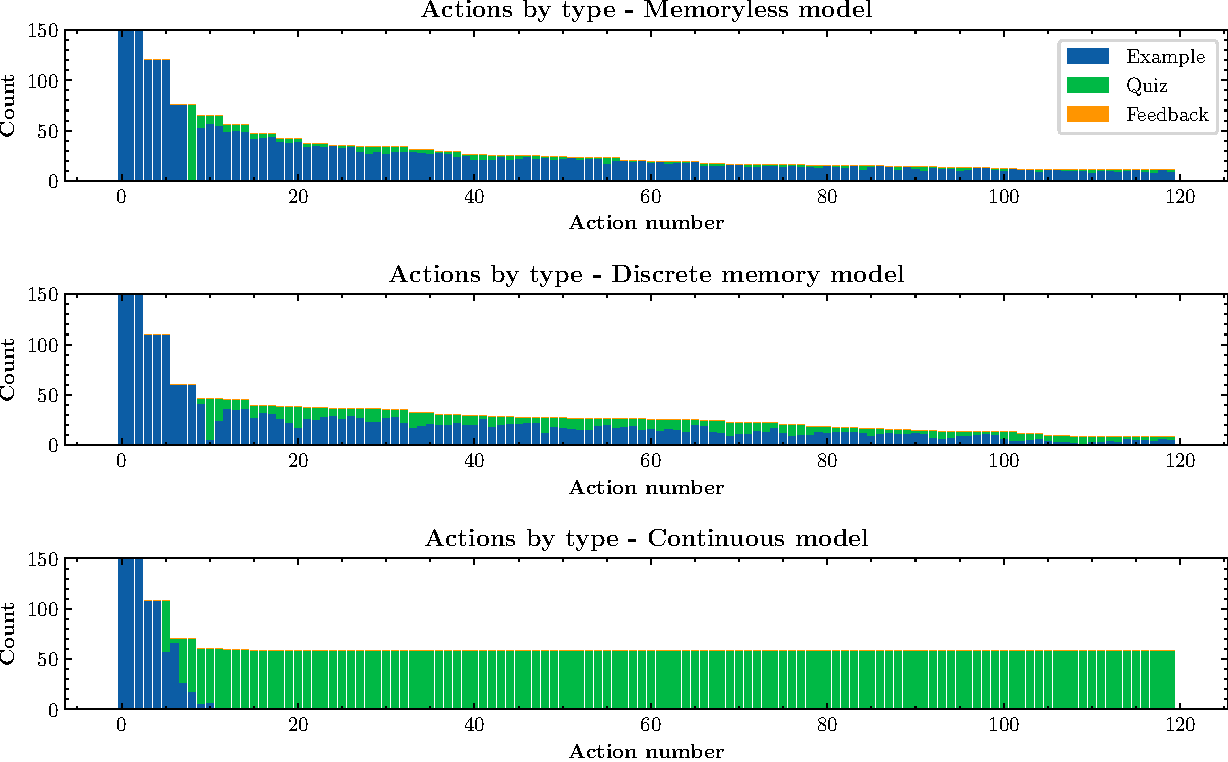
\includegraphics[width=\linewidth]{figures/letter-actions-pre.pdf}
    \caption{Planned activity types per step for each planning model for the letter arithmetic task. 
    %Example actions were predominantly chosen in the discrete models, while the continuous model planned mainly quiz actions after a few steps.
    }
    \label{fig:actions-t1}
\end{figure}

\autoref{fig:actions-t1} shows the teaching activity types planned for each model.
Both the memoryless model and the discrete memory model planned mainly example activities.
Interestingly, both sampled a quiz type after eight and nine example types.
Afterwards, the discrete memory model employed more quizzes than the memoryless model.
The continuous model started with example activities only but gradually used more quiz type actions which were the only type used after action step 12.
No model planned feedback activities.


We provide data tables of the results in the supplementary section \ref{sec:supp}.

\subsubsection{Number game}

% \begin{figure}[t]
%     \centering
%     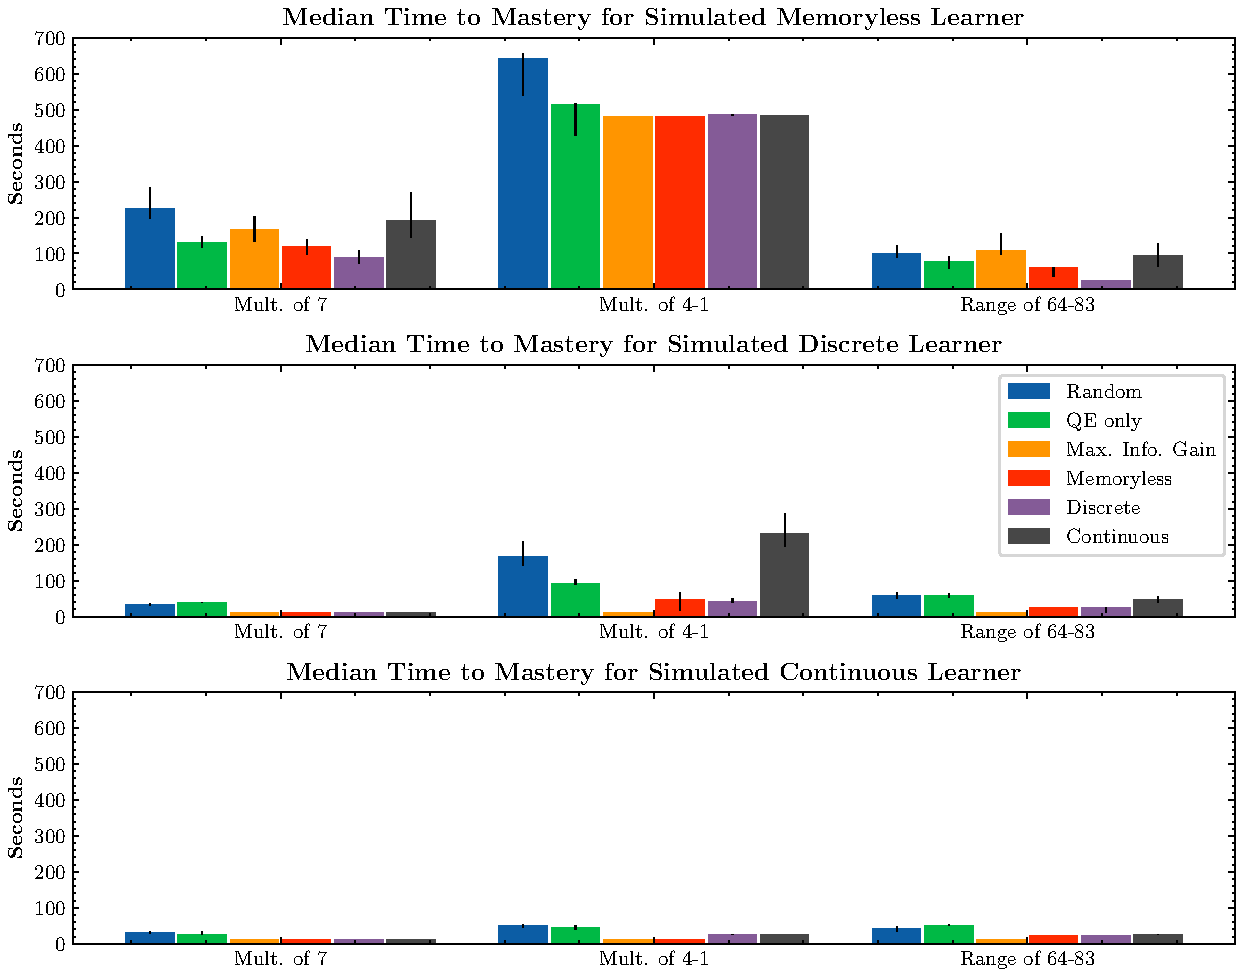
\includegraphics[width=\linewidth]{median-time-ng-combined.pdf}
%     \caption{Median time to mastery for the number game separated for each simulated learner and grouped by task. 
%     Error bars represent bootstrapped 68\% confidence intervals. 
%     Comparable to figure 9 of the original paper.}
%     \label{fig:median-time-ng}
% \end{figure}


% \begin{figure}
%     \centering
%     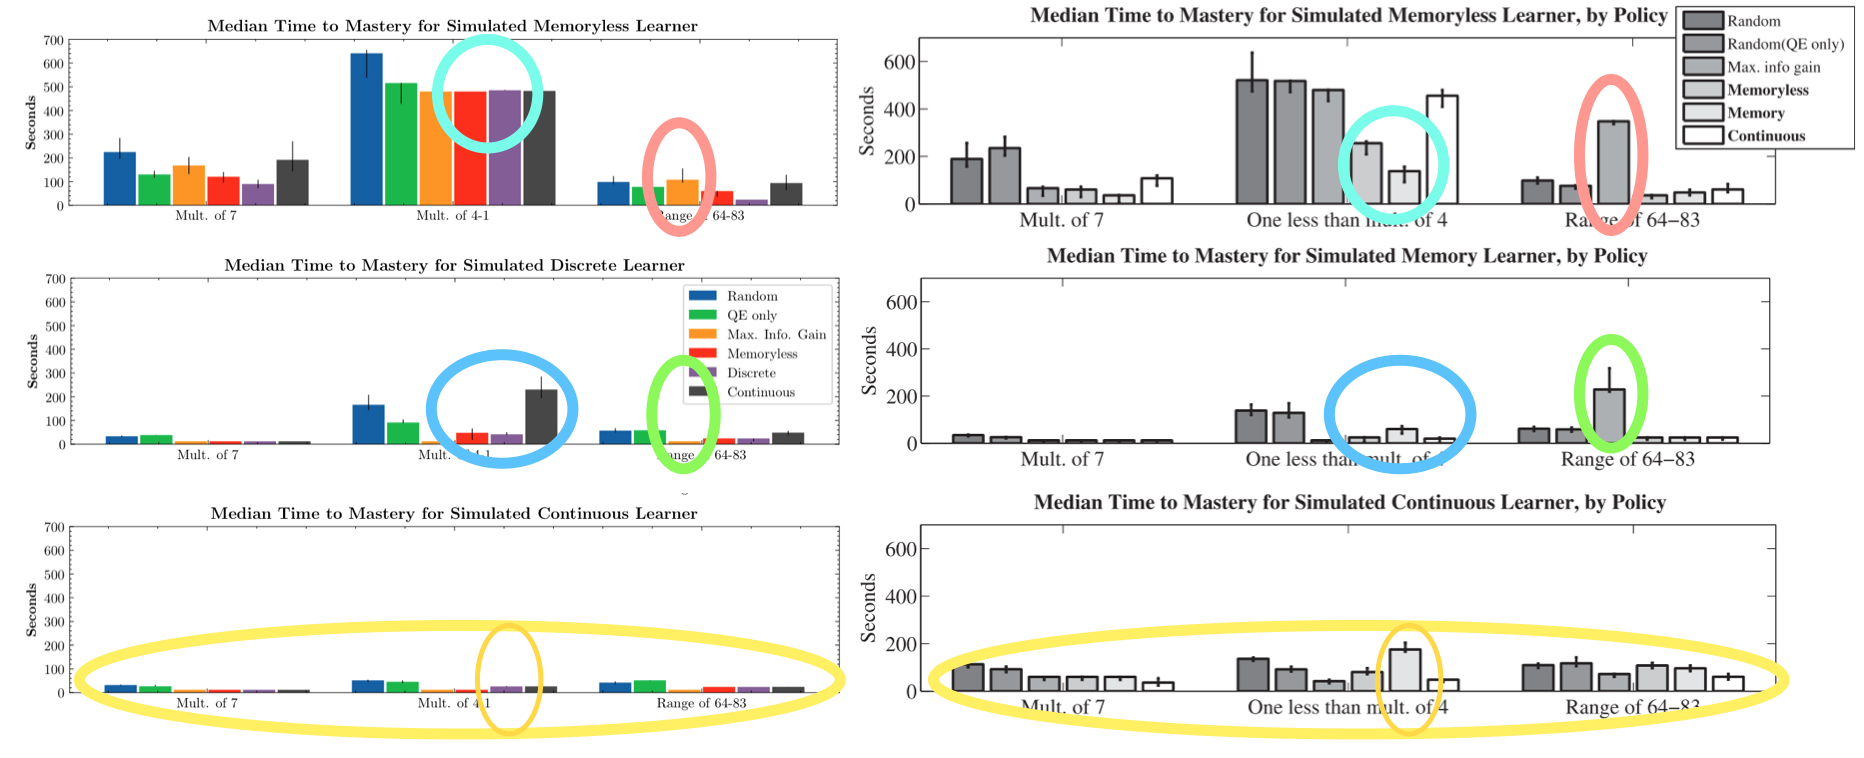
\includegraphics[width=\linewidth]{replication-diff-number-game.png}
%     \caption{Replication difference for the number game between our results (left) and the original data (right).
%     }
%     \label{fig:difference-t2}
% \end{figure}


\begin{figure}
    \centering
    \begin{subfigure}{.9\linewidth}
        \centering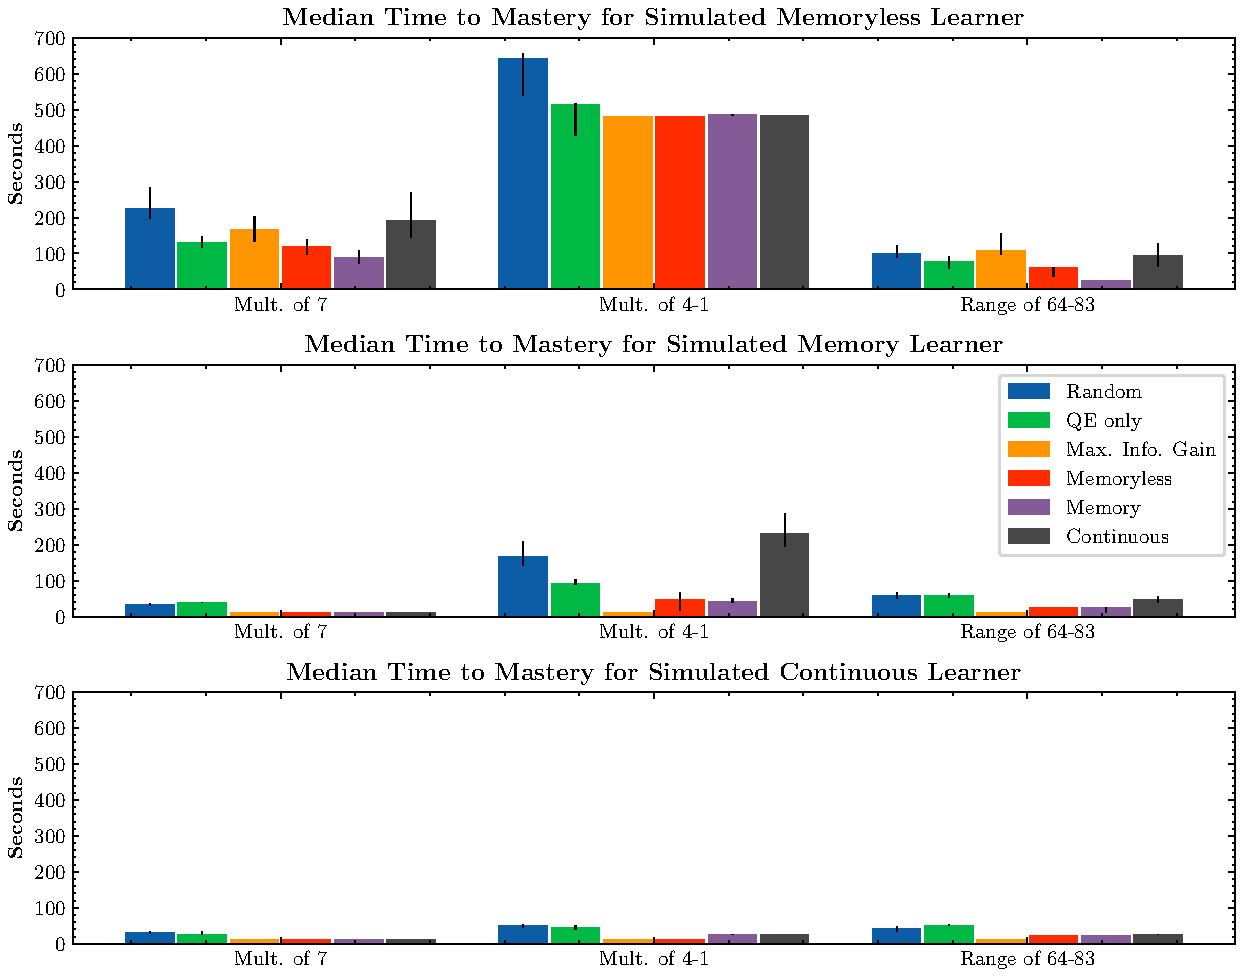
\includegraphics[width=1\linewidth]{figures/median-time-ng-pre.pdf}
        \subcaption{Our results}
    \end{subfigure}
    \vspace{10pt}
     
    \begin{subfigure}{.9\linewidth}
        \centering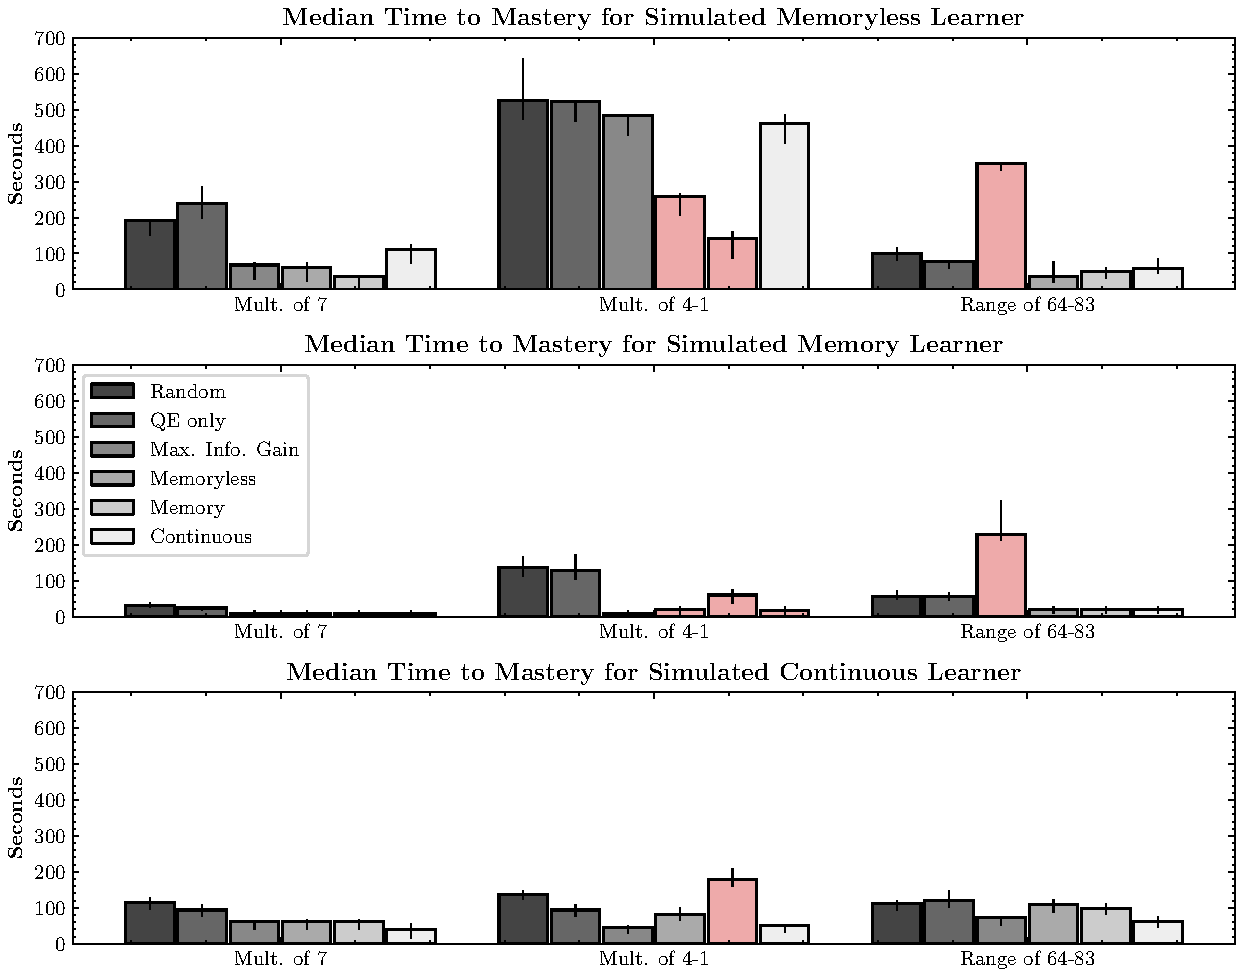
\includegraphics[width=1\linewidth]{figures/median-time-ng-orig.pdf}
        \subcaption{Original results, recreated from original figure 9. Major differences are highlighted in red \\ ($\Delta \geq 50\%$ and relative performance to other policies differs).
        }
    \end{subfigure}
    
    \caption{Median time to mastery for the number game separated for each simulated learner and grouped by task. 
    Error bars represent bootstrapped 68\% confidence intervals. 
    % \textit{Top}: Our results. \textit{Bottom}: Original results, recreated from figure 9 from original paper.
    % TODO define major difference
    }
    \label{fig:median-time-ng-comp}
\end{figure}


Our results are shown in \autoref{fig:median-time-ng-comp} (a). 
The overall structure of the results appear similar to the original results but there are major differences in our data.
We consider differences major if the values differ at least 50\% and the relative performance compared to the other policies is different.

For the simulated memoryless learner (top chart), our results for the target \textit{multiples of 7} are slightly higher and not clearly better than the random policies while their relative performance matches the previously reported results.
For the target \textit{multiples of 4 minus 1}, our results with the memoryless planner and the discrete memory planner differ significantly. 
Our simulations resulted in a median time to mastery of ~480s for both which was reported as ~260s and ~140s in the previous work. 
Hence in our results, no planner exhibits a high performance while previously, the discrete planners resulted in low teaching times.
In the target \textit{Range of 64-83}, we find the maximum information gain policy performs comparable to the continuous policy at 108s while it performed significantly worse than the other planners at ~350s in the original results.

For the simulated discrete memory learner (middle row), with the target \textit{multiples of 4 minus 1}, our continuous planner resulted in a significantly worse performance than all other policies which performed remarkable in the previous paper.
For target \textit{Range of 64-83}, our maximum information gain policy achieves a very high performance with 12s, while in the original results, it was significantly worse than all the other policies with ~230s.

For the simulated continuous learner, we find it to perform significantly better with all targets and with all policies, achieving the best results among the different learners, and not allowing to distinguish between the planners' performance. 
In the original work, the continuous learner was outperformed in many cases by the discrete memory learner and even sometimes the memoryless learner.
For the target \textit{multiples of 4 minus 1}, our policy based on the discrete memory policy performed equally well to the continuous policy with ~26s, while it was previously reported with a performance of ~180s, much higher than the other policies.

In general, we note that our results do not follow a clear line in comparison to the original data.
The best policy for a learner-policy pair is often different in our simulations even if the differences are not large.


\begin{table}
    \centering
    \small
    \begin{tabular}{l|rrr|rrr|rrr|r}
        \hline
        \textbf{Policy} & \multicolumn{3}{l|}{\textbf{Multiples of 7}}  & \multicolumn{3}{l|}{\textbf{Mult. of 4 minus 1}} &  \multicolumn{3}{l|}{\textbf{Range 64-83}} & \textbf{Comp.} \\
                        & Mless & Mem & Cont & Mless & Mem & Cont & Mless & Mem & Cont & \textbf{time} \\
        \hline
        Random          & 12\% & 0\% & 0\% &            54\% & 2\% & 0\% &      2\% & 0\% & 0\% & - \\
        QE only         & 6\% & 0\% & 0\% &            54\% & 2\% & 0\% &      0\% & 0\% & 0\%  & - \\
        \makecell[l]{Max. Info. \\ Gain} & 16\% & 0\% & 0\% &             72\% & 6\% & 0\% &      6\% & 0\% & 0\%  & 0.2s \\
        \hline
        Memoryless      & 4\% & 0\% & 0\% &            70\% & 0\% & 0\% &      0\% & 0\% & 0\%  & 3.7s \\
        Memory          & 4\% & 0\% & 0\% &            70\% & 0\% & 0\% &      0\% & 0\% & 0\%  & 2.4s \\
        Continuous      & 28\% & 0\% & 0\% &           68\% & 18\% & 0\% &       0\% & 0\% & 0\%  & 21.9s \\
        \hline
    \end{tabular}
    \caption{Failure rates and computation times over 50 simulations for the number game tasks. }
    \label{tab:failures-t2}
\end{table}

\autoref{tab:failures-t2} shows the failure rates for the second experiment. 
We note similar results as in the first experiment: The memoryless learner fails to learn in some cases, especially for the target \textit{multiples of 4 minus 1}. In fact, the failure rates are very similar across all planners.
In that task, also the discrete memory learner fails to learn with the random, maximum information gain and continuous policies.
However, the failure rates are lower than in the first experiment.
The continuous learner never fails to learn.


% \begin{table}
% \centering
% \small
% \begin{tabular}{l|r}
% \hline
% \textbf{Model}  & \textbf{Mean computation time}  \\
% \hline
% Max. Info. Gain & 0.2s                  \\
% \hline
% Memoryless      & 3.7s                  \\
% Discrete        & 2.4s                  \\
% Continuous      & 21.92s                  \\
% \hline
% \end{tabular}
% \caption{Planning times for different models for the number game.}
% \label{tab:times-t2}
% \end{table}

The computation times are reported in table \ref{tab:failures-t2} in the last column. 
They are significantly higher than in the first experiment and close or larger than the threshold of 3s. 
In particular, the continuous policy exhibited a mean computation time of more than 20s since it was planning three horizons into the future.
%%% Lukas: In the first task the runtime was never an issue, so I didnt do the cutoff after 3s like they described in the paper. Now I'm thinking for this task it could produce some differences - however overall, for the continuous model the results are close in most cases and rather worse despite the possibly larger search. What do you reckon?
The higher computation times make sense considering that the state space is around 7 times larger than in the letter arithmetic task\footnote{The precomputation times were sometimes significantly higher for the number game, depending on the number of quizzes it sampled in the first 20 steps. This resulted in some cases in over 5,000 paths to be precomputed and a runtime of more than 10 hours. In most cases though, the number of evaluated paths was below 10 and done in few minutes.}.
Note though that we invested less effort into making the computations efficient for the number game.

\begin{figure}
    \centering
    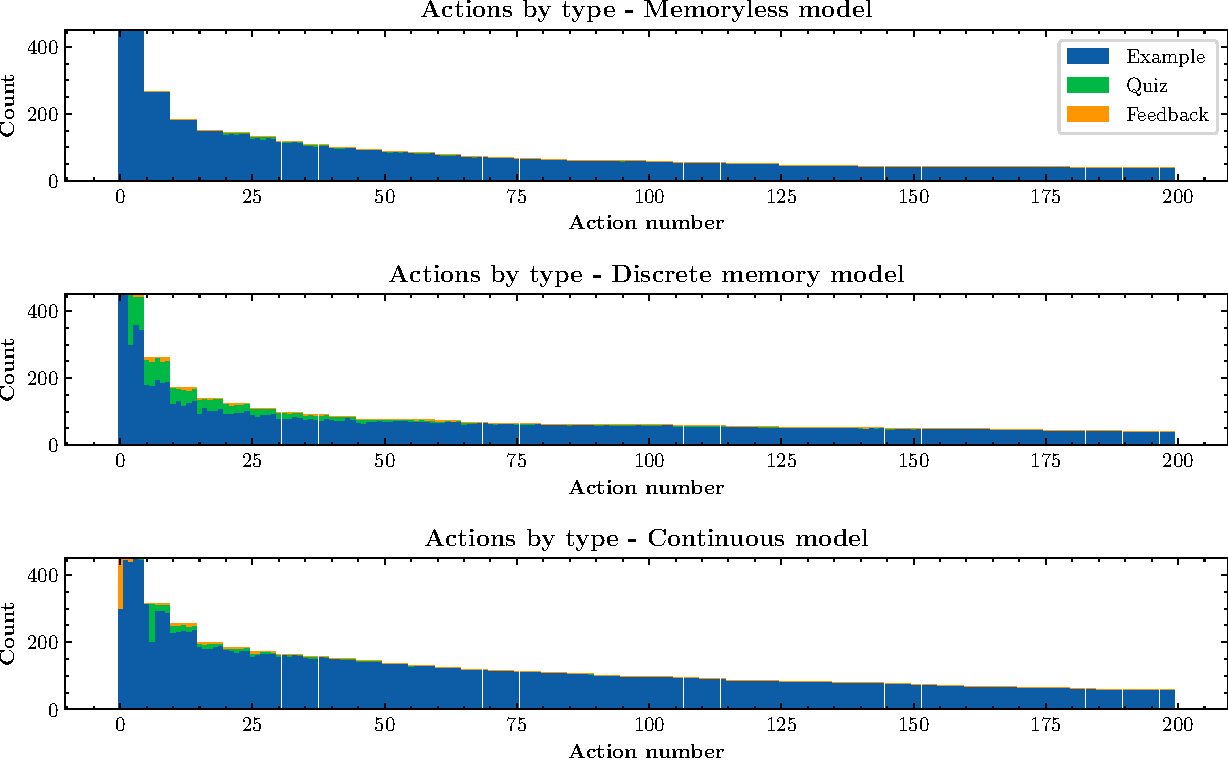
\includegraphics[width=\linewidth]{figures/ng-actions-pre.pdf}
    \caption{Planned teaching activity types per step for each planning model for the number game. 
    %Example actions were predominantly chosen.
    }
    \label{fig:actions-t2}
\end{figure}

Finally, \autoref{fig:actions-t2} shows the sampled teaching types for the different models, combined for all three tasks.
Recall that in the number game, the cheapest action type was the example action.
We notice that it is strongly dominated by example actions in all planners.
The discrete memory and the continuous model sometimes planned feedback actions and quiz actions.

Again, detailed results and statistics are provided in the supplementary section \ref{sec:supp}.

\subsection{Implementation}

We implemented the model in Python 3, using Numpy to perform many calculations in vectorized form.
Simulations are run in parallel to reduce the needed execution time. 
Reproducibility is achieved by using fixed seeds for the random number generators in Python and Numpy. 
The code is publicly available on GitHub at \url{https://github.com/luksurious/faster-teaching/}. 
All possible execution modes are configurable via command-line arguments which also allows a manual learning mode for diagnosis. 

All simulations were executed on Ubuntu 18.04 with Python 3.7.5 on an Intel(R) Xeon(R) CPU E5-1650 v4 @ 3.60GHz and 32GB of RAM.

To improve performance, the belief update is always performed separately for refinement and evidence activities as described before. 
Further, the planning algorithm is slightly improved to stop the iteration over possible observations if the current cost of the action is already higher than the currently known best value.
% Note though, that the code for the letter arithmetic task is more optimized than the code for the number game.

To handle edge cases where a belief contains zero probability for all concepts (usually due to inconsistent responses), we reset the belief in the discrete models to the initial belief, similar to the particle depletion case in the particle filter implementation.

%In the random policy, to achieve a sensible baseline, we ensure that the same item is not used in a single teaching phase.

The biggest difference to the original implementation is that we did not employ the limit on the computation times to 3s since we did not perform a user study.
